\section{Roles} The role itself is a collection of permissions. To decide what roles the application needs and what permissions those roles would have, we have to start by analyzing the users of the application and their needs. My analysis will be based on the existing roles and access control system.\\
Since it is the best practice to assign as few roles to one user as it is possible \cite{role-auth} to avoid creating an excessively complex management system I will aim for simplification of the current access control system. In this section I will describe the roles of the current BI-DBS portal and offer a simplification for the new application, which I will use for my implementation of role-based access control described in section 4.3.

\subsection{KOS roles}
The BI-DBS portal receives information about an authorized user from the study information system(KOS) based on the course information. The course information contains the identifier of the semester and the type of study program. Generally, there are seven user roles that are defined by the KOS for subjects and courses.\cite{kosapi}\\

\noindent \textbf{KOS roles for subjects and their general description:\cite{kosroles}}

\begin{itemize}
    \item \emph{Guarantor.} Guarantor is a course administrator. Thus a person with this role typically has all permissions across all course management.
    \item \emph{Examiner.} Examiners are responsible for managing and estimating students' exams. Therefore, this role would usually provide access to exam materials and students' grades view and management.
    \item \emph{Editor.} Editor is a person who can edit the information about the subject. This role would provide access to subject information management.
    \item \emph{Lecturer.} Lecturer role indicates that an individual with this role would need to be provided with access to manage course content including lectures, assignments and other study materials.
    \item \emph{Instructor.} Instructor is the role for teachers of exercises parallels. This role implies that a user needs permission to manage exercise materials and also estimate students' tests, semester works and other assignments.
    \item \emph{Teacher.} The teacher is a general role for a person, who does teaching in the course. 
    \item \emph{Student.} It is a base role for students, that usually grants basic permissions to a user like access to their personal information, study program information and its resources, and also allows managing their projects and submitting assignments.
\end{itemize}


\noindent One of those roles is not used for the BI-DBS portal. It is the editor role, the BI-DBS portal does not provide functionalities for changing the information about the subject. Therefore, we have a total of six roles used for permissions control in the current application.\\  
Based on the feedback from the teachers and developers of the current BI-DBS portal and also my own research, we came to the conclusion that the access management system can be simplified by grouping the roles into three roles in total.\\

\noindent \textbf{Reasons for simplifying the access management:}

\begin{enumerate}
    \item Based on the permissions research of the current project, I can report that most of the roles for teachers have the same or almost the same permissions. And the differences are insignificant.
    \item All the analyses and requirements of the BI-DBS portal designed by students including the theses are made for only three roles.
    \item Due to a lack of information about the roles developers often do not have a good understanding of all roles meaning and thus they tend to forget to permit access for some roles or confuse them with others.
\end{enumerate}

\noindent I am offering the simplification, which is based on grouping teaching roles that do not have significant permissions differences such as lecturer, examiner, instructor and teacher into one role. As I have already mentioned above, all the analyses are usually built on three roles where these 4 roles are taken as one role - teacher role, then there is a student and guarantor roles left which makes it a total of three.\\

\begin{figure}[h]
\centering
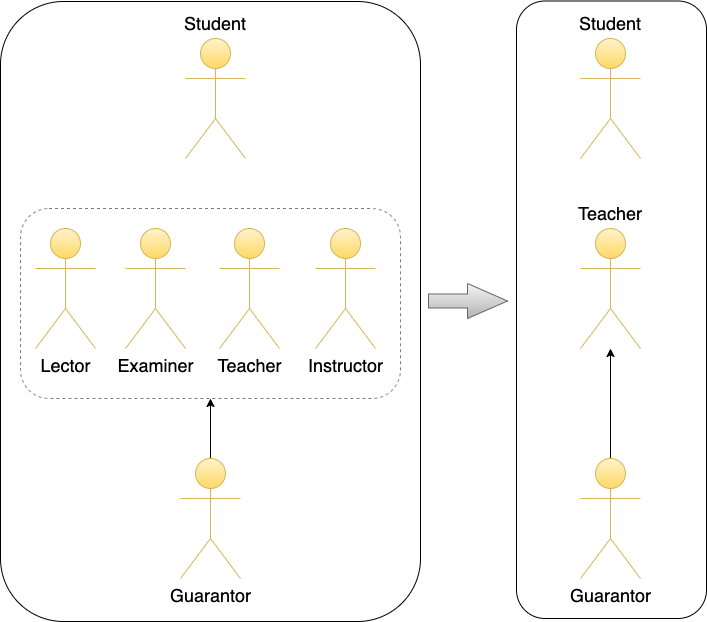
\includegraphics[scale=0.52]{../png/kos_roles.png}
\caption{KOS roles}\label{picture:kos_roles}
\end{figure}


\noindent After researching the functionalities and permissions structure of the current project and discussing the possible change with developers and managers, I came to the conclusion that it is absolutely safe to generalize the permissions for those four teacher roles. As a result, I got a new clear KOS roles structure, which is visualized in Figure 3.1.




\subsection{Other roles}

\noindent However, the user roles defined by KOS are not fulfilling all the requirements for the application. There are some special cases that require additional roles such as:

\begin{itemize}
    \item \emph{Impersonation as a student.} For the purpose of demonstrating the process of creating a semestral work and its management, teachers need to have a functionality that will allow them to authorize as a student to show the whole process from the students' side. This feature requires creating a test student, which is identical to a usual student but needs  to differ from the usual KOS student role to exclude such student records from counting the statistics. 
    \item \emph{Development and testing.} For the development and testing processes there is a need to have a test admin user, which will have access to all functionalities. 
\end{itemize}

\begin{figure}[h]
\centering
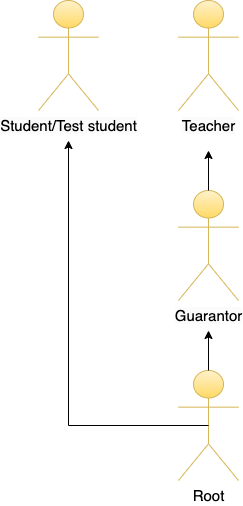
\includegraphics[scale=0.54]{../png/roles.png}
\caption{Other roles}\label{picture:special_roles}
\end{figure}


\noindent For these requirements there were created two corresponding special roles:

\begin{itemize}
    \item \emph{Test student.} This role is identical to the KOS student role from the perspective of permissions. Therefore on the frontend we do not need to differ those two roles and the student test role will be mapped to a usual student role.
    \item \emph{Admin.} Role with access to all functionalities.
\end{itemize}

\noindent Conclusively, the solution for the access control system lowered complexity and added flexibility, due to the rule that one user can have only one role. Besides, now the roles system is very intuitive in usage. The result of constructing a roles system for the role-based access control is visualized in Figure 3.2.
